\documentclass[10pt,a4paper,fleqn]{article}
\usepackage[utf8]{inputenc}
\usepackage[portuguese]{babel}
\usepackage[T1]{fontenc}
\usepackage{amsmath}
\usepackage{amsfonts}
\usepackage{amssymb}
\usepackage{graphicx}
\usepackage{setspace}

\title{Disciplina M\'{e}todos Potenciais}
\author{Vanderlei C. Oliveira Jr.}
\date{}

\doublespace

\begin{document}

\begin{flushleft}
\begin{huge}
\emph{Disciplina M\'{e}todos Potenciais}
\end{huge}
\end{flushleft}
\begin{flushleft}
Vanderlei C. Oliveira Jr. \\
Observat\'{o}rio Nacional - MCTI \\
Rio de Janeiro - 2014
\end{flushleft}

\hrulefill

\tableofcontents

\hrulefill

%%%%%%%%%%%%%% Funções harmônicas %%%%%%%%%%%%%%
%%%%%%%%%%%%%%%%%%%%%%%%%%%%%%%%%%%%%%%%%%%%%%%%
\section{Funç\~{o}es harm\^{o}nicas}

%%%%% Exercício 11 %%%%%
\subsection{Funç\~{a}o potencial magn\'{e}tico escalar}

Seja $f(x,y,z)$ dada por
\begin{equation}
f(x,y,z) = - \iiint \limits_{v} \mathbf{m}(x',y',z')^{\intercal}
                                \left( \nabla \frac{1}{r} \right)
                                 d v \quad
\label{eq:ex11-func-f}
\end{equation}
em que $r = \sqrt{(x-x')^{2}+(y-y')^{2}+(z-z')^{2}}$ \'{e} a dist\^{a}ncia entre o ponto $(x,y,z)$
e o ponto $(x',y',z')$ dentro do volume de integraç\~{a}o $v$ (Figura \ref{fig:fig1}). Os vetores
$\mathbf{m}(x',y',z')$ e $\nabla \frac{1}{r}$ s\~{a}o dados por
\begin{equation}
\mathbf{m}(x',y',z') =
\left[
\begin{array}{c}
m_{x}(x',y',z') \\
m_{y}(x',y',z') \\
m_{z}(x',y',z')
\end{array}
\right]_{3 \times 1}
\label{eq:ex11-mag-vec}
\end{equation}
e
\begin{equation}
\nabla \frac{1}{r} =
\left[
\begin{array}{c}
\frac{\partial}{\partial x} \frac{1}{r} \\
\frac{\partial}{\partial y} \frac{1}{r} \\
\frac{\partial}{\partial z} \frac{1}{r}
\end{array}
\right]_{3 \times 1} \quad .
\label{eq:ex11-grad-invr}
\end{equation}

\begin{flushleft}
\dotfill
\end{flushleft}

\subsubsection{Exerc\'{i}cio}

Mostre que a funç\~{a}o $f(x,y,z)$ (Eq. \ref{eq:ex11-func-f}) \'{e} harm\^{o}nica e, portanto, satisfaz
a equaç\~{a}o de Laplace em coordenadas Cartesianas
\begin{equation}
\frac{\partial^{2} f(x,y,z)}{\partial x^{2}} +
\frac{\partial^{2} f(x,y,z)}{\partial y^{2}} +
\frac{\partial^{2} f(x,y,z)}{\partial z^{2}} = 0 \quad .
\label{eq:ex11-Laplace}
\end{equation}

\begin{flushleft}
\dotfill
\end{flushleft}

%Figuras ==>
\begin{figure}[h]
    \centering
    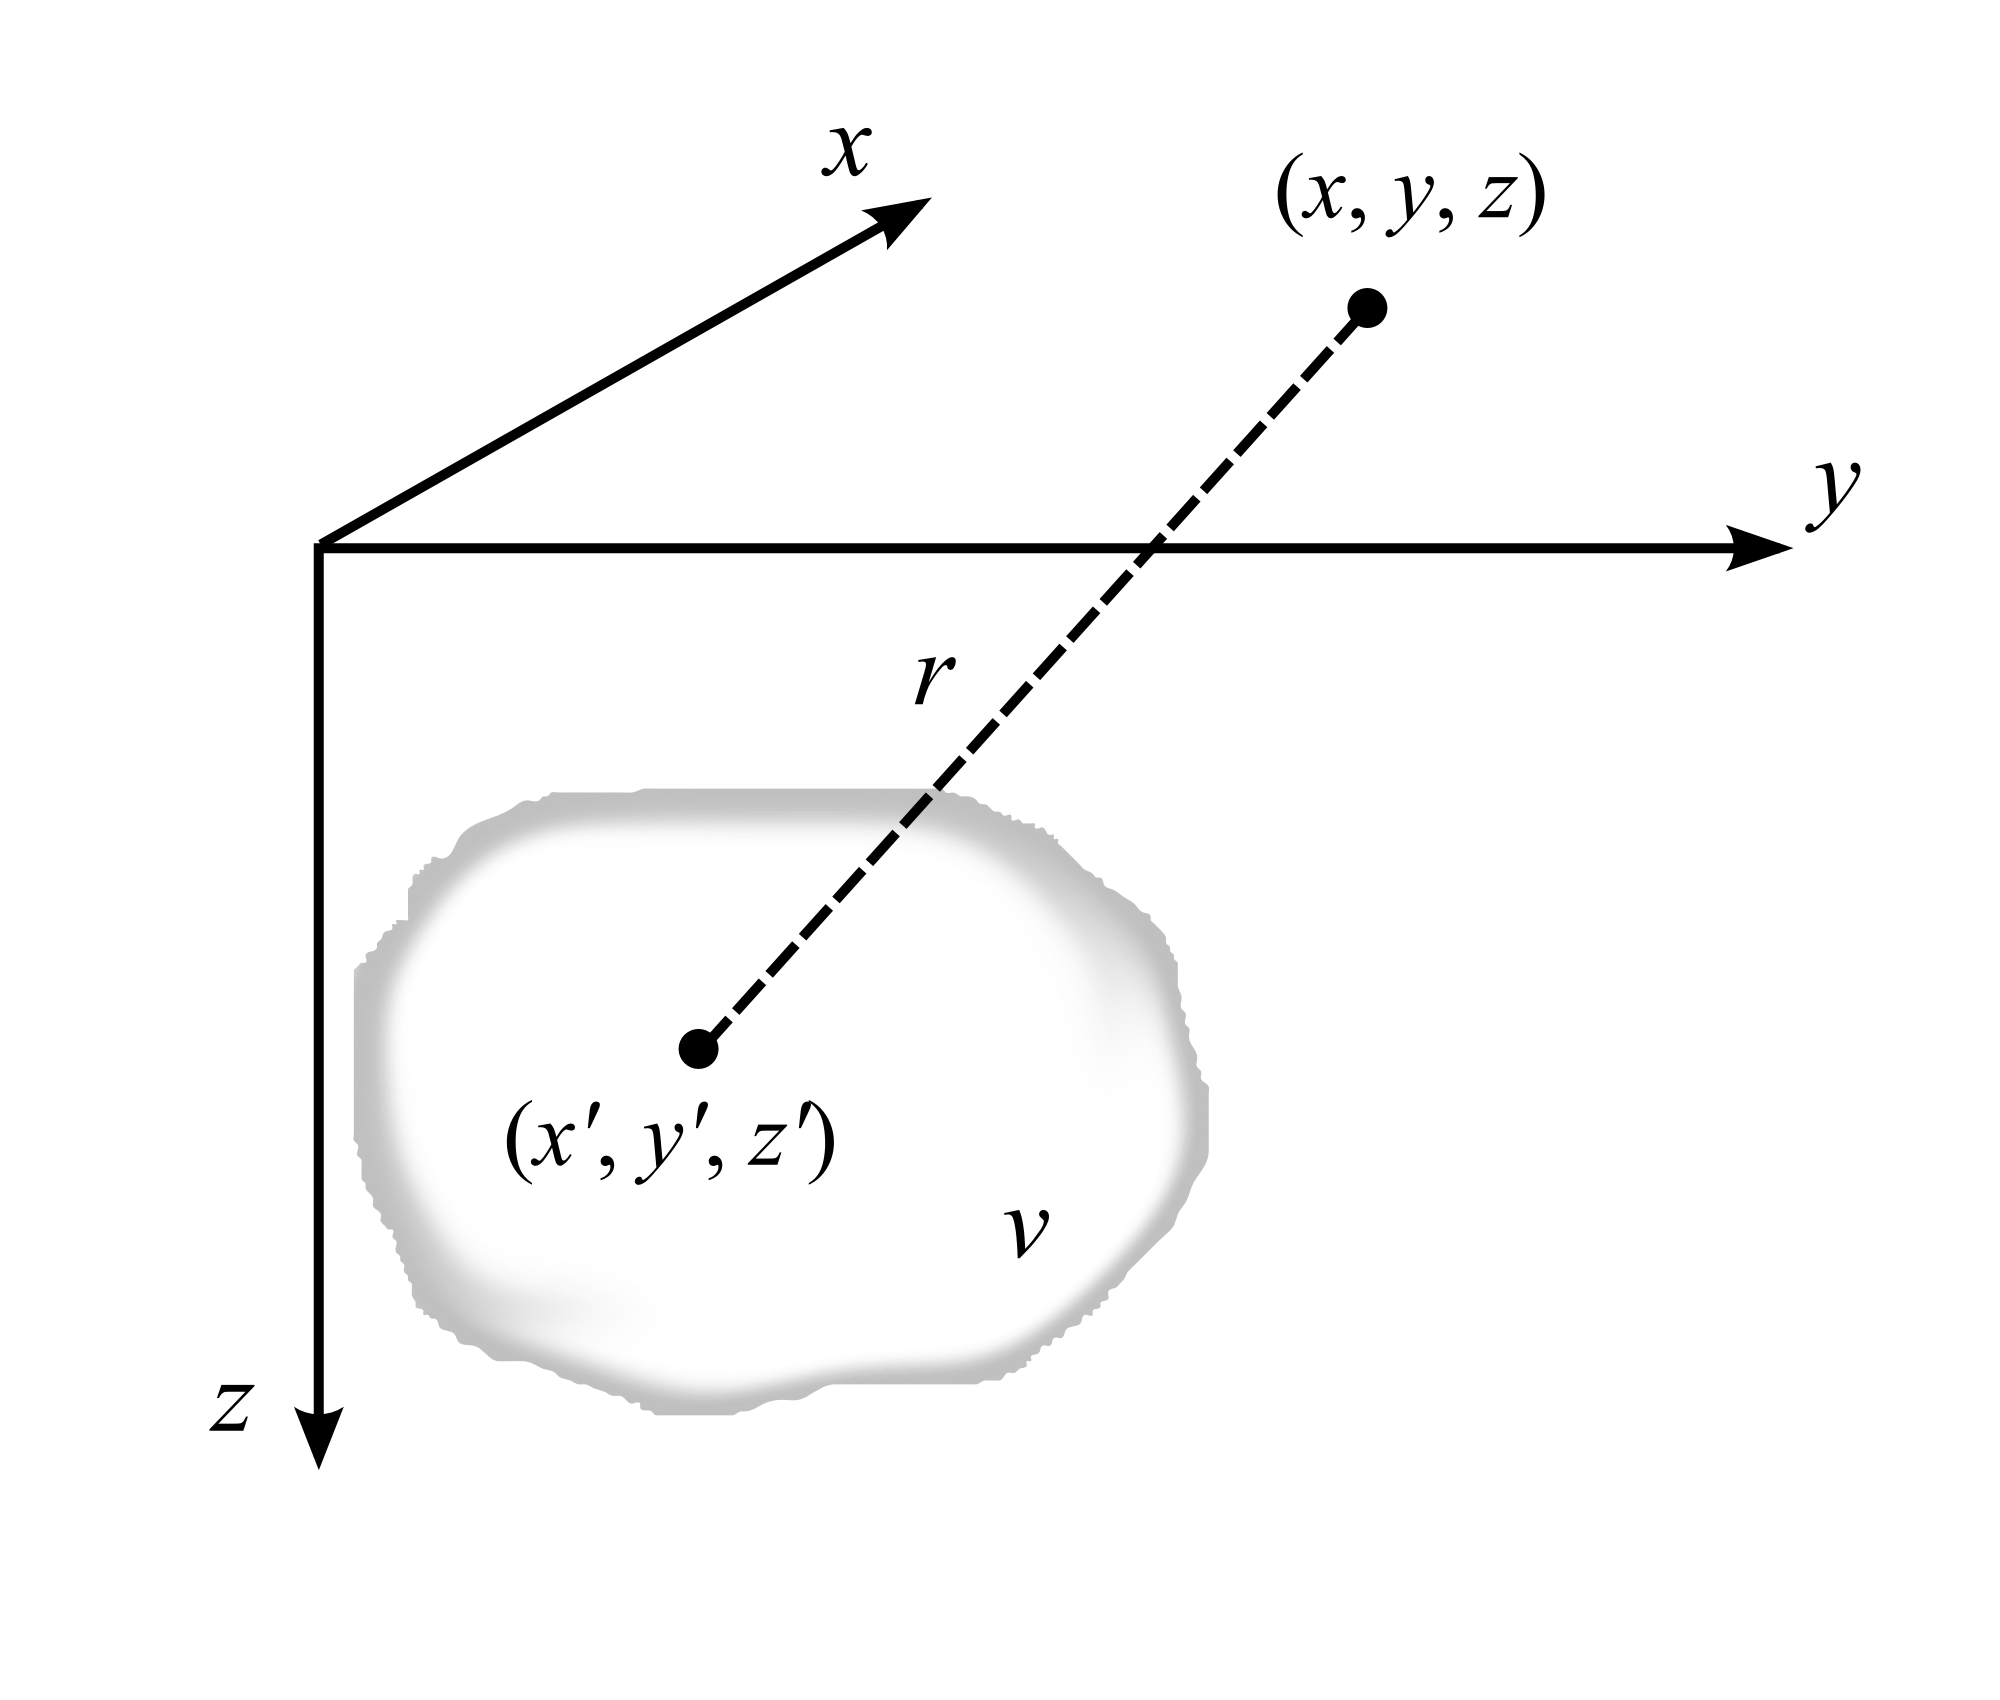
\includegraphics[scale=1]{Figs/Fig1.png}
    \caption{Dist\^{a}ncia $r = \sqrt{(x-x')^{2}+(y-y')^{2}+(z-z')^{2}}$ entre
        um ponto $(x,y,z)$ e outro ponto $(x',y',z')$ de um sistema de coordenadas Cartesianas. O ponto
        $(x',y',z')$ est\'{a} dentro do volume de integraç\~{a}o $v$.}   
    \label{fig:fig1}
\end{figure}
%<== Figuras

%%%%%%%%%%%%%% Harmônicos esféricos %%%%%%%%%%%%%%
%%%%%%%%%%%%%%%%%%%%%%%%%%%%%%%%%%%%%%%%%%%%%%%%%%
\section{Harm\^{o}nicos esf\'{e}ricos}

%%%%% Exercício 2.1 %%%%%
\subsection{Equaç\~{o}es diferenciais de $r$}

Sejam $f_{1}(r)$ e $f_{2}(r)$ duas funç\~{o}es dadas por
\begin{equation}
f_{1}(r) = r^{n}
\label{eq:ex211-r^}
\end{equation}
e
\begin{equation}
f_{2}(r) = r^{-(n+1)} \quad ,
\label{eq:ex211-r_}
\end{equation}
em que $n \geqslant 0$ \'{e} um n\'{u}mero inteiro e $r > 0$ \'{e} um n\'{u}mero real. 

\begin{flushleft}
\dotfill
\end{flushleft}

\subsubsection{Exerc\'{i}cio}

Mostre que $f_{1}(r)$ (Eq. \ref{eq:ex211-r^}) e $f_{2}(r)$ (Eq. \ref{eq:ex211-r_}) 
s\~{a}o soluç\~{o}es da equaç\~{a}o diferencial
\begin{equation}
r^{2} \: \frac{d^{2} f(r)}{d r^{2}} + 2 \: r \: \frac{d \, f(r)}{d r} - n(n+1) \: f(r) = 0 \quad .
\label{eq:ex211-eqdif-r}
\end{equation}

\begin{flushleft}
\dotfill
\end{flushleft}

%%%%% Exercício 2.2 %%%%%
\subsection{Equaç\~{o}es diferenciais de $\lambda$}

Sejam $h_{1}(\lambda)$ e $h_{2}(\lambda)$ duas funç\~{o}es dadas por
\begin{equation}
h_{1}(\lambda) = cos(m \lambda)
\label{eq:ex212-cos}
\end{equation}
e
\begin{equation}
h_{2}(\lambda) = sen(m \lambda) \quad ,
\label{eq:ex212-sen}
\end{equation}
em que $m \geqslant 0$ \'{e} um n\'{u}mero inteiro e $\lambda$ \'{e} um n\'{u}mero real. 

\begin{flushleft}
\dotfill
\end{flushleft}

\subsubsection{Exerc\'{i}cio}

Mostre que
$h_{1}(\lambda)$ (Eq. \ref{eq:ex212-cos}) e $h_{2}(\lambda)$ (Eq. \ref{eq:ex212-sen}) 
s\~{a}o soluç\~{o}es da equaç\~{a}o diferencial
\begin{equation}
\frac{d^{2} h(\lambda)}{d \lambda^{2}} + m^{2} h(\lambda) = 0 \quad .
\label{eq:ex212-eqdif-lamb}
\end{equation}

\begin{flushleft}
\dotfill
\end{flushleft}

%%%%% Exercício 2.3 %%%%%
\subsection{Polin\^{o}mios de Legendre}

A equaç\~{a}o diferencial
\begin{equation}
sen \theta \, g''(\theta) + 
cos \theta \, g'(\theta) + 
\left[ n(n+1) \, sen \theta - \dfrac{m^{2}}{sen \theta} \right] = 0
\label{eq:ex213-eq-diff-Legendre-theta}
\end{equation}
tem como soluç\~{a}o os polin\^{o}mios associados de Legendre
\begin{equation}
g(\theta) = P_{nm}(cos\theta) \quad .
\label{eq:ex213-g-theta}
\end{equation}
Nestas Equaç\~{o}es, $n$ e $m$ s\~{a}o inteiros maiores ou iguais a zero (sendo $m$ menor ou igual a $n$), 
$g'(\theta)$ \'{e} a primeira derivada e $g''(\theta)$ \'{e} a segunda derivada de $g(\theta)$. Os inteiros $n$ 
e $m$ s\~{a}o, respectivamente, o grau e a ordem do polin\^{o}mio $P_{nm}(cos\theta)$. Por conveni\^{e}ncia, 
estas Equaç\~{o}es s\~{a}o comumente transformadas por mudança de vari\'{a}veis  utilizando a relaç\~{a}o 
$t = cos{\theta}$. Dessa forma,
\begin{equation}
\begin{array}{l}
g(\theta) = \overline{g}(t) \\
g'(\theta) = -\overline{g}'(t) \, sen \theta \\
g''(\theta) = \overline{g}''(t) \, sen^{2} \theta - \overline{g}'(t) \, cos \theta \quad .
\end{array}
\label{eq:ex213-g-t}
\end{equation}
em que $\overline{g}(t) = P_{nm}(t)$, com primeira e segunda derivadas $\overline{g}'(t)$ e $\overline{g}''(t)$, 
respectivamente. Substituindo as Equaç\~{o}es \ref{eq:ex213-g-t} na equaç\~{a}o diferencial 
\ref{eq:ex213-eq-diff-Legendre-theta}, dividindo o resultado por $sen \theta$ e utilizando a relaç\~{a}o $sen^{2} 
\theta = 1 - t^2$ temos que
\begin{equation}
(1 - t^2) \, \overline{g}''(t) - 2 \, t \, \overline{g}'(t) +
\left[ n(n+1) - \frac{m^{2}}{1 - t^2} \right] = 0 \quad .
\label{eq:ex213-eq-diff-Legendre-t}
\end{equation}
A funç\~{a}o $\overline{g}(t) = P_{nm}(t)$ (polin\^{o}mio associado de Legendre escrito em funç\~{a}o da viari\'{a}vel 
$t$) que satisfaz a Equaç\~{a}o \ref{eq:ex213-eq-diff-Legendre-t} pode ser dada por
\begin{equation}
P_{nm}(t) = \frac{1}{2^{n} \, n!} \, (1 - t^{2})^{m/2} \,
\frac{d^{n+m}}{d \, t^{n+m}}(t^{2} - 1)^{n} \quad .
\label{eq:ex213-pnm-t}
\end{equation}
Por exemplo,
\begin{equation}
\begin{split}
P_{11}(t) & = \frac{(1 - t^{2})^{1/2}}{2} \, \frac{d^{2}}{d \, t^{2}}(t^{2} - 1) \\
& = \sqrt{1 - t^{2}} \\
& = sen \theta \quad ,
\end{split}
\label{eq:ex213-p11-t}
\end{equation}
ou
\begin{equation}
\begin{split}
P_{21}(t) & = \frac{(1 - t^{2})^{1/2}}{2^{2} \, 2!} \, \frac{d^{3}}{d \, t^{3}}(t^{2} - 1)^{2} \\
& = \frac{\sqrt{1 - t^{2}}}{8} \, (16 \, t + 8 \, t) \\
& = 3 \, t \, \sqrt{1 - t^{2}} \\
& = 3 \, sen \theta \, cos \theta \quad .
\end{split}
\label{eq:ex213-p21-t}
\end{equation}
No caso particular em que $m = 0$, n\~{a}o h\'{a} ra\'{i}zes $\sqrt{1 - t^{2}}$, $P_{nm}(t)$ \'{e} representado 
simplesmente por $P_{n}(t)$ e \'{e} denominado polin\^{o}mio de Legendre. A partir da Equação \ref{eq:ex213-pnm-t}, 
os polin\^{o}mios de Legendre podem ser escritos como
\begin{equation}
P_{n}(t) = \frac{1}{2^{n} \, n!} \frac{d^{n}}{d \, t^{n}}(t^{2} - 1)^{n} \quad .
\label{eq:ex213-pn-t}
\end{equation}
Alternativamente, os polin\^{o}mios de Legendre (\ref{eq:ex213-pn-t}) a partir do grau $n = 2$ podem ser obtidos pela 
f\'{o}rmula recursiva
\begin{equation}
P_{n}(t) = - \, \frac{n - 1}{n} \, P_{n-2}(t) + \frac{2n - 1}{n} \, t \, P_{n-1}(t) \quad ,
\label{eq:ex213-pn-recursiva}
\end{equation}
em que $P_{2}(t)$ \'{e} obtido utilizando $P_{0}(t)$ e $P_{1}(t)$, $P_{3}(t)$ \'{e} obtido utilizando $P_{1}(t)$ e $P_{2}(t)$, etc.

\begin{flushleft}
\dotfill
\end{flushleft}

\subsubsection{Exerc\'{i}cio}

Determine os polin\^{o}mios associados de Legendre de grau $n = 0$ e ordem $m = 0$ at\'{e} grau $n = 3$ 
e ordem $m = 3$ utilizando a Equação \ref{eq:ex213-pnm-t}.

\subsubsection{Exerc\'{i}cio}

Determine os polin\^{o}mios de Legendre de grau $n = 0$ at\'{e} $n = 5$ utilizando a Equação \ref{eq:ex213-pn-t}. Em seguida, determine os polin\^{o}mios de grau $n = 2$ at\'{e} $n = 5$ utilizando a f\'{o}rmula recursiva 
(Eq. \ref{eq:ex213-pn-recursiva}). Por último, faça um gr\'{a}fico dos polin\^{o}mios de Legendre $P_{n}(t)$ de grau 
$n = 0$ at\'{e} $n = 5$ para $t$ no intervalo $[-1,1]$. 

\begin{flushleft}
\dotfill
\end{flushleft}

%%%%% Exercício 2.4 %%%%%
\subsection{Equaç\~{a}o de Laplace em coordenadas esf\'{e}ricas}

Seja $V(r,\theta,\lambda)$ uma funç\~{a}o harm\^{o}nica que depende das coordenadas esf\'{e}ricas $r$, $\theta$ e $\lambda$ 
(Fig. \ref{fig:fig2}). Esta funç\~{a}o satisfaz a equaç\~{a}o de Laplace em coordenadas esf\'{e}ricas, que pode ser escrita como
\begin{equation}
r^{2} \, \frac{\partial^{2} \, V}{\partial \, r^{2}} +
2 \, r \, \frac{\partial \, V}{\partial \, r} +
\frac{\partial^{2} \, V}{\partial \, \theta^{2}} +
cot \theta \, \frac{\partial \, V}{\partial \, \theta} +
\frac{1}{sen^{2} \theta} \, \frac{\partial^{2} \, V}{\partial \, \lambda^{2}} = 0 \quad .
\label{eq:ex214-eq-Laplace-esferica}
\end{equation}

%Figuras ==>
\begin{figure}[h]
    \centering
    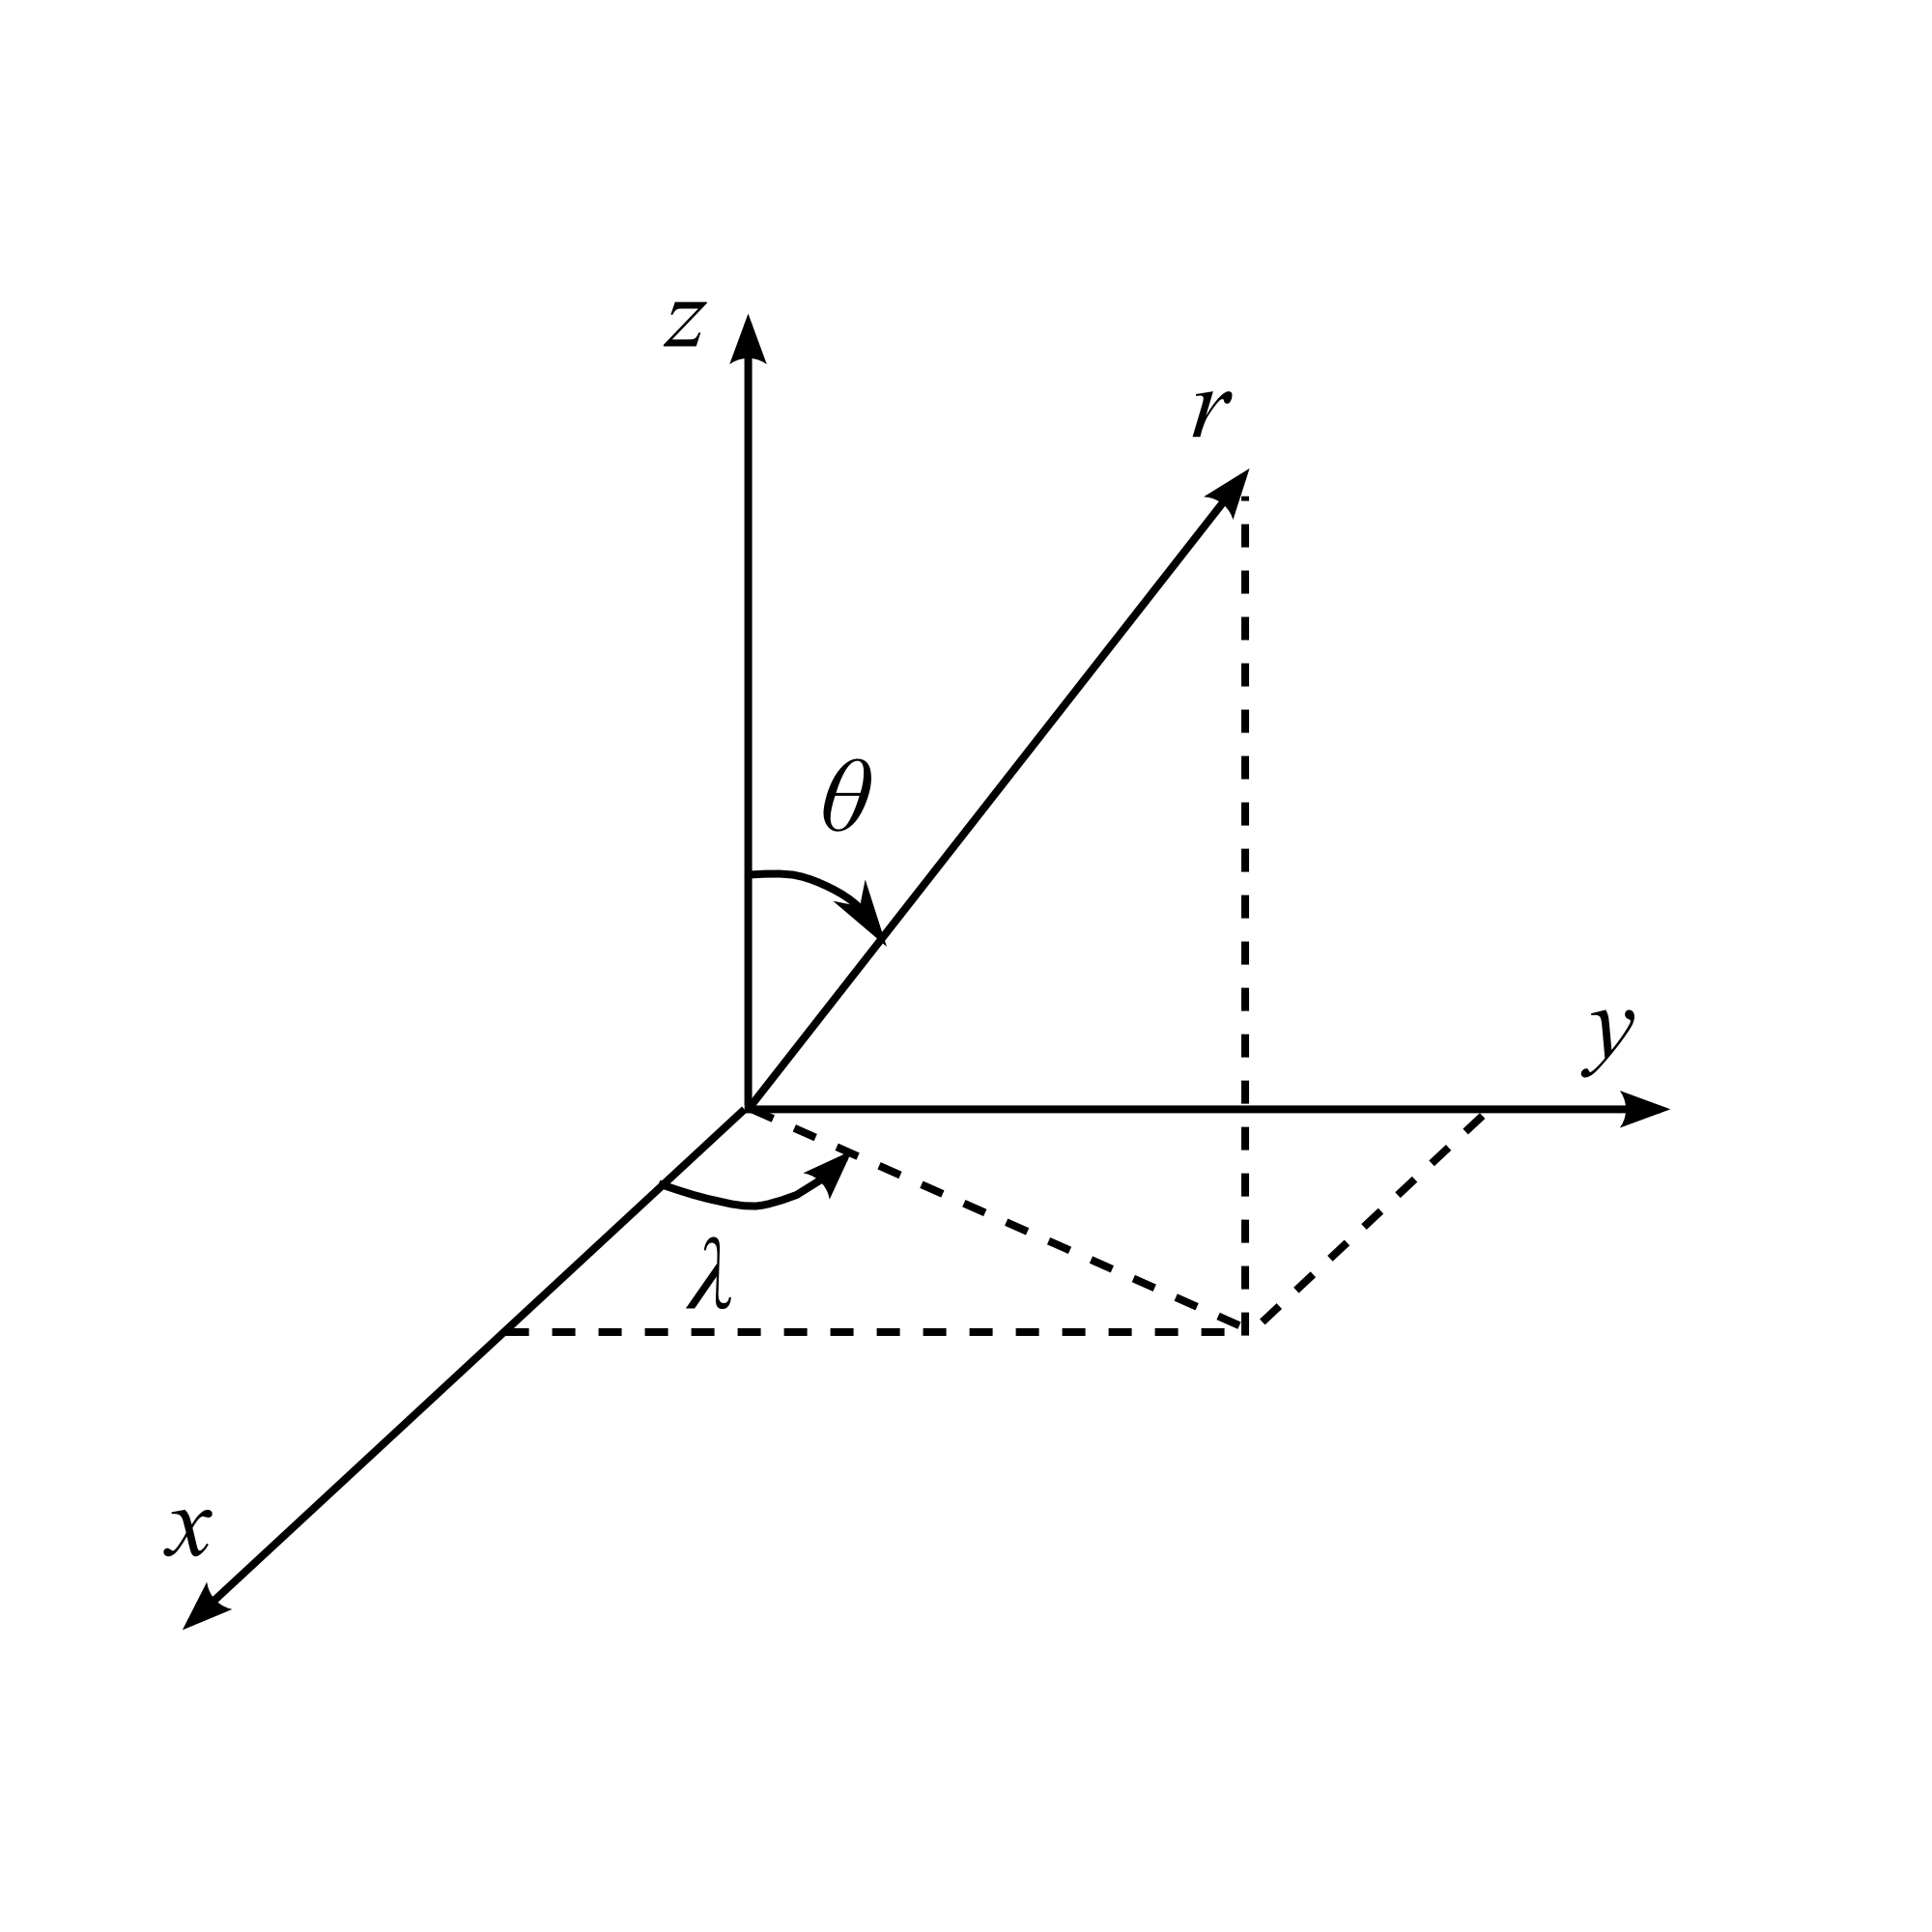
\includegraphics[scale=1]{Figs/Fig2.png}
    \caption{Sistema de coordenadas Cartesianas $(x,y,z)$ e esf\'{e}ricas $(r,\theta,\lambda)$.}
    \label{fig:fig2}
\end{figure}
%<== Figuras

\bigskip
\bigskip

\begin{flushleft}
\emph{\textbf{Soluç\~{a}o da Equaç\~{a}o de Laplace em coordenadas esf\'{e}ricas}}
\end{flushleft}

\bigskip
\bigskip

A equação de Laplace \ref{eq:ex214-eq-Laplace-esferica} pode ser resolvida pelo m\'{e}todo de separaç\~{a}o de vari\'{a}veis. 
Este m\'{e}todo consiste em supor que a funç\~{a}o $V(r,\theta,\lambda)$ pode ser reescrita como o produto entre tr\^{e}s funç\~{o}es 
independentes:
\begin{equation}
V(r,\theta,\lambda) = f(r) \, g(\theta) \, h(\lambda) \quad .
\label{eq:ex214-v-fhg}
\end{equation}
O pr\'{o}ximo passo consiste em determinar as funç\~{o}es $f(r)$, $g(\theta)$ e $h(\lambda)$. Para tanto, basta substituir a funç\~{a}o 
$V(r,\theta,\lambda)$ dada pela Equaç\~{a}o \ref{eq:ex214-v-fhg} na equaç\~{a}o de Laplace \ref{eq:ex214-eq-Laplace-esferica}. Esta 
substituiç\~{a}o nos leva a conclus\~{a}o de que a funç\~{a}o $f(r)$ (Eq. \ref{eq:ex214-v-fhg}) satisfaz a equaç\~{a}o diferencial 
\ref{eq:ex211-eqdif-r}. Tal como visto anteriormente, as funç\~{o}es $f_{1}(r)$ (Eq. \ref{eq:ex211-r^}) e $f_{2}(r)$ 
(Eq. \ref{eq:ex211-r_}) s\~{a}o soluç\~{o}es desta equaç\~{a}o. Neste caso, mostra-se que a funç\~{a}o $V(r,\theta,\lambda)$ pode 
ser escrita como:
\begin{equation}
V(r,\theta,\lambda) = r^{n} \, g(\theta) \, h(\lambda) \quad ,
\label{eq:ex214-v-f1gh}
\end{equation}
ou
\begin{equation}
V(r,\theta,\lambda) = \frac{1}{r^{(n+1)}} \, g(\theta) \, h(\lambda) \quad .
\label{eq:ex214-v-f2gh}
\end{equation}
Estas funç\~{o}es s\~{a}o denominadas harm\^{o}nicos esf\'{e}ricos s\'{o}lidos. De forma an\'{a}loga, mostra-se que a funç\~{a}o 
$h(\lambda)$ (Eq. \ref{eq:ex214-v-fhg}) satisfaz a equaç\~{a}o diferencial \ref{eq:ex212-eqdif-lamb}, que possui as soluç\~{o}es 
$h_{1}(\lambda)$ (Eq. \ref{eq:ex212-cos}) e $h_{2}(\lambda)$ (Eq. \ref{eq:ex212-sen}), e que a funç\~{a}o $g(\theta)$ (Eq. 
\ref{eq:ex214-v-fhg}) satisfaz a equaç\~{a}o diferencial \ref{eq:ex213-eq-diff-Legendre-theta}, cuja soluç\~{a}o \'{e} dada 
pelos polin\^{o}mios associados de Legendre $P_{nm}(cos\theta)$ (Eq. \ref{eq:ex213-g-theta}). Os polin\^{o}mios associados de 
Legendre $P_{nm}(cos\theta)$ podem ser obtidos pela Equação \ref{eq:ex213-pnm-t}, em que $t = cos \theta$. Por fim, \'{e} poss\'{i}vel 
mostrar que a funç\~{a}o $V(r,\theta,\lambda)$ pode ser escrita de duas formas:
\begin{equation}
V_{e}(r,\theta,\lambda) = \sum_{n=0}^{\infty} r^{n} \, 
Y_{n}(\theta, \lambda) \quad ,
\label{eq:ex214-ve}
\end{equation}
ou
\begin{equation}
V_{i}(r,\theta,\lambda) = \sum_{n=0}^{\infty} \frac{1}{r^{(n+1)}} \,
Y_{n}(\theta, \lambda) \quad ,
\label{eq:ex214-vi}
\end{equation}
em que 
\begin{equation}
Y_{n}(\theta, \lambda) = \sum_{m=0}^{n} 
\left[ 
A_{nm} \, R_{nm}(\theta, \lambda) +
B_{nm} \, S_{nm}(\theta, \lambda)
\right] \quad ,
\label{eq:ex214-Yn}
\end{equation}
sendo $A_{nm}$ e $B_{nm}$ constantes e as funç\~{o}es $R_{nm}(\theta, \lambda)$ e $S_{nm}(\theta, \lambda)$ dadas por
\begin{equation}
R_{nm}(\theta, \lambda) = P_{nm}(cos\theta) \, cos(m \, \lambda)
\label{eq:ex214-rnm}
\end{equation}
e
\begin{equation}
S_{nm}(\theta, \lambda) = P_{nm}(cos\theta) \, sen(m \, \lambda) \quad .
\label{eq:ex214-snm}
\end{equation}
As funç\~{o}es $Y_{n}(\theta, \lambda)$ (Eq. \ref{eq:ex214-Yn}) s\~{a}o denominadas harm\^{o}nicos (esf\'{e}ricos) de superf\'{i}cie.

\bigskip
\bigskip

\begin{flushleft}
\emph{\textbf{Relaç\~{o}es de ortogonalidade entre as funç\~{o}es $R_{nm}(\theta, \lambda)$ e $S_{nm}(\theta, \lambda)$}}
\end{flushleft}

\bigskip
\bigskip

As constantes $A_{nm}$ e $B_{nm}$ (Eq. \ref{eq:ex214-Yn}) podem ser determinadas por meio das relaç\~{o}es de ortogonalidade entre as
funç\~{o}es $R_{nm}(\theta, \lambda)$ (Eq. \ref{eq:ex214-rnm}) e $S_{nm}(\theta, \lambda)$ (Eq. \ref{eq:ex214-snm}). Para tanto, vamos
considerar $r = 1$ nas equaç\~{o}es \ref{eq:ex214-ve} e \ref{eq:ex214-vi}. Dessa maneira, estas equaç\~{o}es s\~{a}o iguais a uma funç\~{a}o 
$f(\theta,\lambda)$ que pode ser escrita em funç\~{a}o dos harm\^{o}nicos de superf\'{i}cie (Eq. \ref{eq:ex214-Yn}) da seguinte forma
\begin{equation}
\begin{split}
f(\theta,\lambda) & = \sum_{n=0}^{\infty} 
Y_{n}(\theta, \lambda) \\
& = \sum_{n=0}^{\infty} \,
\sum_{m=0}^{n} \left[ 
A_{nm} \, R_{nm}(\theta, \lambda) +
B_{nm} \, S_{nm}(\theta, \lambda)
\right] \: .
\end{split}
\label{eq:ex214-f}
\end{equation}
De acordo com as relaç\~{o}es de ortogonalidade entre as funç\~{o}es $R_{nm}(\theta, \lambda)$ (Eq. \ref{eq:ex214-rnm}) e 
$S_{nm}(\theta, \lambda)$ (Eq. \ref{eq:ex214-snm}),
\begin{equation}
\iint \limits_{\sigma}
R_{nm}(\theta, \lambda) \, R_{op}(\theta, \lambda) \, d \sigma  = 0
\label{eq:ex214-ortog-rnm}
\end{equation}
e
\begin{equation}
\iint \limits_{\sigma}
S_{nm}(\theta, \lambda) \, S_{op}(\theta, \lambda) \, d \sigma = 0
\label{eq:ex214-ortog-snm}
\end{equation}
para o caso em que $nm \neq op$. J\'{a} a integral
\begin{equation}
\iint \limits_{\sigma}
R_{nm}(\theta, \lambda) \, S_{op}(\theta, \lambda) \, d \sigma  = 0
\label{eq:ex214-ortog-rnm-snm}
\end{equation}
\'{e} sempre zero, independente dos valores de $o$ e $p$. Nestas Equaç\~{o}es, 
$\iint \limits_{\sigma} = \int_{\lambda = 0}^{2\pi} \, \int_{\theta = 0}^{\pi}$ e $d 
\sigma = sen\theta \, d\theta d\lambda$. Por outro lado, estas integrais s\~{a}o diferentes 
de zero quando $nm = op$. Neste caso,
\begin{equation}
\iint \limits_{\sigma}
R_{n0}^{2}(\theta, \lambda) \, d \sigma  = \dfrac{4 \, \pi}{2 \, n + 1}
\label{eq:ex214-ortog-rn02}
\end{equation}
e
\begin{equation}
\left.
\begin{array}{l}
\iint \limits_{\sigma}
R_{nm}^{2}(\theta, \lambda) \, d \sigma \\
\iint \limits_{\sigma}
S_{nm}^{2}(\theta, \lambda) \, d \sigma
\end{array}
\right \} =
\dfrac{2 \, \pi}{2 \, n + 1} \dfrac{(n + m)!}{(n - m)!} \: .
\label{eq:ex214-ortog-rnm2-snm2}
\end{equation}
Observe que estas integrais (Eqs. \ref{eq:ex214-ortog-rnm}, \ref{eq:ex214-ortog-snm}, \ref{eq:ex214-ortog-rnm-snm},
\ref{eq:ex214-ortog-rn02} e \ref{eq:ex214-ortog-rnm2-snm2}) s\~{a}o avaliadas sobre a superf\'{i}cie $\sigma$ de uma esfera
com raio unit\'{a}rio, cuja \'{a}rea \'{e} igual a $4 \, \pi$.

\bigskip
\bigskip

\begin{flushleft}
\emph{\textbf{Determinaç\~{a}o das constantes $A_{nm}$ e $B_{nm}$}}
\end{flushleft}

\bigskip
\bigskip

Para determinar as constantes $A_{nm}$ (Eqs. \ref{eq:ex214-Yn} e \ref{eq:ex214-f}), basta multiplicar os 
dois lados da Equação \ref{eq:ex214-f} por $R_{op}(\theta,\lambda)$ (Eq. \ref{eq:ex214-rnm}), integrar o resultado sobre 
a superf\'{i}cie $\sigma$ de uma esfera com raio unit\'{a}rio e utilizar as relaç\~{o}es de ortogonalidade 
(Eqs. \ref{eq:ex214-ortog-rnm}, \ref{eq:ex214-ortog-snm}, \ref{eq:ex214-ortog-rnm-snm}, \ref{eq:ex214-ortog-rn02} e 
\ref{eq:ex214-ortog-rnm2-snm2}):
\begin{equation}
\begin{split}
R_{op}(\theta,\lambda) \, f(\theta,\lambda)
& = R_{op}(\theta,\lambda) \, \sum_{n=0}^{\infty} \,
\sum_{m=0}^{n} \left[ 
A_{nm} \, R_{nm}(\theta, \lambda) +
B_{nm} \, S_{nm}(\theta, \lambda)
\right] \\
& \begin{array}{r} =
\left[ A_{00} \, R_{op}(\theta,\lambda) \, R_{00}(\theta, \lambda) \right. + \\
B_{00} \, R_{op}(\theta,\lambda) \, S_{00}(\theta, \lambda) + \\
A_{10} \, R_{op}(\theta,\lambda) \, R_{10}(\theta, \lambda) + \\
B_{10} \, R_{op}(\theta,\lambda) \, S_{10}(\theta, \lambda) + \\
A_{11} \, R_{op}(\theta,\lambda) \, R_{11}(\theta, \lambda) + \\
B_{11} \, R_{op}(\theta,\lambda) \, S_{11}(\theta, \lambda) + \\
\vdots \quad \quad \quad \quad \quad \\
A_{op} \, R_{op}(\theta,\lambda) \, R_{op}(\theta, \lambda) + \\
B_{op} \, R_{op}(\theta,\lambda) \, S_{op}(\theta, \lambda) + \\
\vdots \quad \quad \quad \quad \quad \\
A_{nn} \, R_{op}(\theta,\lambda) \, R_{nn}(\theta, \lambda) + \\
\left. B_{nn} \, R_{op}(\theta,\lambda) \, S_{nn}(\theta, \lambda) \right]
\end{array} \\
& = \left[ \, \hdots + A_{op} \, R_{op}^{2}(\theta,\lambda) + \hdots \, \right]
\end{split}
\label{eq:ex214-int-Anm-desenvolv}
\end{equation}

\begin{equation}
\begin{split}
\iint \limits_{\sigma} 
f(\theta,\lambda) \, R_{op}(\theta,\lambda) \, d \sigma
& = \left[ \, \hdots + 
\iint \limits_{\sigma} A_{op} \, R_{op}^{2}(\theta,\lambda) \, d \sigma
+ \hdots \, \right] \\
& = \left[ \, \hdots + 
A_{op} \, \iint \limits_{\sigma} R_{op}^{2}(\theta,\lambda) \, d \sigma
+ \hdots \, \right] \\
& = 
A_{op} \, \iint \limits_{\sigma} R_{op}^{2}(\theta,\lambda) \, d \sigma
\end{split} \: .
\label{eq:ex214-int-Anm}
\end{equation}

De forma an\'{a}loga, para determinar as constantes $B_{nm}$ (Eqs. \ref{eq:ex214-Yn} e \ref{eq:ex214-f}), basta multiplicar os 
dois lados da Equação \ref{eq:ex214-f} por $S_{op}(\theta,\lambda)$ (Eq. \ref{eq:ex214-snm}), integrar o resultado sobre a 
superf\'{i}cie $\sigma$ de uma esfera com raio unit\'{a}rio e utilizar as relaç\~{o}es de ortogonalidade 
(Eqs. \ref{eq:ex214-ortog-rnm}, \ref{eq:ex214-ortog-snm}, \ref{eq:ex214-ortog-rnm-snm}, \ref{eq:ex214-ortog-rn02} e 
\ref{eq:ex214-ortog-rnm2-snm2}):
\begin{equation}
\iint \limits_{\sigma} 
f(\theta,\lambda) \, S_{op}(\theta,\lambda) \, d \sigma
= B_{op} \, \iint \limits_{\sigma} S_{op}^{2}(\theta,\lambda) \, d \sigma \: .
\label{eq:ex214-int-Bnm}
\end{equation}
A partir das Equaç\~{o}es \ref{eq:ex214-int-Anm} e \ref{eq:ex214-int-Bnm} temos que
\begin{equation}
A_{n0} = \dfrac{2 \, n + 1}{4 \, \pi} \, 
\iint \limits_{\sigma} 
f(\theta,\lambda) \, R_{n0}(\theta,\lambda) \, d \sigma \; ,
\label{eq:ex214-An0}
\end{equation}
\begin{equation}
A_{nm} = \dfrac{2 \, n + 1}{2 \, \pi} \, \dfrac{(n - m)!}{(n + m)!} \,
\iint \limits_{\sigma} 
f(\theta,\lambda) \, R_{nm}(\theta,\lambda) \, d \sigma \; , \: m \neq 0 \, ,
\label{eq:ex214-Anm}
\end{equation}
e
\begin{equation}
B_{nm} = \dfrac{2 \, n + 1}{2 \, \pi} \, \dfrac{(n - m)!}{(n + m)!} \,
\iint \limits_{\sigma} 
f(\theta,\lambda) \, S_{nm}(\theta,\lambda) \, d \sigma \; , \: m \neq 0 \, .
\label{eq:ex214-Anm}
\end{equation}

\bigskip
\bigskip

\begin{flushleft}
\emph{\textbf{Normalizaç\~{a}o das funç\~{o}es $R_{nm}(\theta, \lambda)$ e $S_{nm}(\theta, \lambda)$}}
\end{flushleft}

\bigskip
\bigskip

Em geof\'{i}sica, a descriç\~{a}o do campo de gravidade e do campo geomagn\'{e}tico \'{e} feita por
meio dos harm\^{o}nicos esf\'{e}ricos (Eqs. \ref{eq:ex214-ve} e \ref{eq:ex214-vi}). Contudo, por 
conveni\^{e}ncia, a descriç\~{a}o destes campos n\~{a}o \'{e} feita utilizando-se as funç\~{o}es 
$R_{nm}(\theta, \lambda)$ (Eq. \ref{eq:ex214-ortog-rnm}) e $S_{nm}(\theta, \lambda)$ 
(Eq. \ref{eq:ex214-ortog-snm}). Ao inv\'{e}s destas funç\~{o}es, s\~{a}o utilizadas as funç\~{o}es 
normalizadas
\begin{equation}
\overline{R}_{nm}(\theta,\lambda) = c_{nm} \, R_{nm}(\theta,\lambda)
\label{eq:ex214-rnm-norm}
\end{equation}
e
\begin{equation}
\overline{S}_{nm}(\theta,\lambda) = c_{nm} \, S_{nm}(\theta,\lambda) \: .
\label{eq:ex214-snm-norm}
\end{equation}
Para descrever o campo de gravidade, os coeficientes $c_{nm}$ 
(Eqs. \ref{eq:ex214-rnm-norm} e \ref{eq:ex214-snm-norm}) são 
\begin{equation}
c_{n0}^{gr} = \sqrt{2 \, n + 1}
\label{eq:ex214-cn0-grav}
\end{equation}
e
\begin{equation}
c_{nm}^{gr} = \sqrt{2 \, (2 \, n + 1) \, \dfrac{(n - m)!}{(n + m)!}} \: , \quad m \neq 0 \, .
\label{eq:ex214-cnm-grav}
\end{equation}
Para descrever o campo geomagn\'{e}tco, os coeficientes $c_{nm}$ 
(Eqs. \ref{eq:ex214-rnm-norm} e \ref{eq:ex214-snm-norm}) são 
\begin{equation}
c_{n0}^{ge} = 1
\label{eq:ex214-cn0-geom}
\end{equation}
e
\begin{equation}
c_{nm}^{ge} = \sqrt{2 \, \dfrac{(n - m)!}{(n + m)!}} \: , \quad m \neq 0 \, .
\label{eq:ex214-cnm-geom}
\end{equation}

\begin{flushleft}
\dotfill
\end{flushleft}

\subsubsection{Exerc\'{i}cio}

Utilizando as relaç\~{o}es de ortogonalidade entre as funç\~{o}es $R_{nm}(\theta, \lambda)$ 
(Eq. \ref{eq:ex214-ortog-rnm}) e $S_{nm}(\theta, \lambda)$ (Eq. \ref{eq:ex214-ortog-snm}),
determine 
$$\dfrac{1}{4 \, \pi} \, \iint \limits_{\sigma} \left[ \overline{R}_{nm}^{gr} (\theta, \lambda)
\right]^{2} \, d \sigma \: ,$$ 
$$\dfrac{1}{4 \, \pi} \, \iint \limits_{\sigma} \left[ \overline{S}_{nm}^{gr} (\theta, \lambda)
\right]^{2} \, d \sigma \: ,$$ 
$$\dfrac{1}{4 \, \pi} \, \iint \limits_{\sigma} \left[ \overline{R}_{nm}^{ge} (\theta, \lambda)
\right]^{2} \, d \sigma$$ 
e
$$\dfrac{1}{4 \, \pi} \, \iint \limits_{\sigma} \left[ \overline{S}_{nm}^{ge}  (\theta, \lambda)
\right]^{2} \, d \sigma \: ,$$
em que $\iint \limits_{\sigma} = \int_{\lambda = 0}^{2\pi} \, \int_{\theta = 0}^{\pi}$ e $d \sigma 
= sen\theta \, d\theta d\lambda$. Nestas integrais, $\overline{R}_{nm}^{gr} (\theta, \lambda)$ e 
$\overline{S}_{nm}^{gr} (\theta, \lambda)$ representam as funç\~{o}es normalizadas $\overline{R}_{nm}
(\theta, \lambda)$ (Eq. \ref{eq:ex214-rnm-norm}) e $\overline{S}_{nm} (\theta, \lambda)$ 
(Eq. \ref{eq:ex214-snm-norm}) utilizando-se os coeficientes $c_{n0}^{gr}$ (Eq. \ref{eq:ex214-cn0-grav}) 
e $c_{nm}^{gr}$ (Eq. \ref{eq:ex214-cnm-grav}). Analogamente, $\overline{R}_{nm}^{ge} (\theta, \lambda)$ 
e $\overline{S}_{nm}^{ge} (\theta, \lambda)$ representam as funç\~{o}es normalizadas 
$\overline{R}_{nm} (\theta, \lambda)$ (Eq. \ref{eq:ex214-rnm-norm}) e $\overline{S}_{nm} (\theta, \lambda)$ 
(Eq. \ref{eq:ex214-snm-norm}) utilizando-se os coeficientes $c_{n0}^{ge}$ 
(Eq. \ref{eq:ex214-cn0-geom}) e $c_{nm}^{ge}$ (Eq. \ref{eq:ex214-cnm-geom}).

\begin{flushleft}
\dotfill
\end{flushleft}

\bigskip
\bigskip

\begin{flushleft}
\emph{\textbf{Expans\~{a}o da funç\~{a}o inverso da dist\^{a}ncia e f\'{o}rmula da decomposiç\~{a}o}}
\end{flushleft}

\bigskip
\bigskip

%%%%%%%%%%%% Anomalia de Campo Total%%%%%%%%%%%%%%
%%%%%%%%%%%%%%%%%%%%%%%%%%%%%%%%%%%%%%%%%%%%%%%%%%
\section{Anomalia de Campo Total}

\subsection{Definiç\~{a}o}

Considere uma \'{a}rea de estudo sobre uma pequena região na superfície do planeta. 
Em um dado intervalo curto de tempo, podemos considerar que a parcela do campo 
geomagnético que é produzida pelo n\'{u}cleo da Terra é 
um vetor constante em toda a \'{a}rea de estudo. Este vetor pode ser escrito como
\begin{equation}
\mathbf{F} = \| \mathbf{F} \| \, \hat{\mathbf{F}} \; ,
\label{eq:campo-geomagnetico}
\end{equation}
em que $\| \mathbf{F} \|$ é a intensidade de $\mathbf{F}$ e $\hat{\mathbf{F}}$ é um vetor unitário
dado por
\begin{equation}
\hat{\mathbf{F}} = \left[
\begin{array}{c}
cos(I) \, cos(D) \\
cos(I) \, sen(D) \\
sen(I)
\end{array}
\right] \; ,
\label{eq:versor-campo-geomagnetico}
\end{equation}
sendo $D$ e $I$ a declinação e a inclinação de $\mathbf{F}$, respectivamente, de 
acordo com a Figura \ref{fig:fig3}.

%Figuras ==>
\begin{figure}[h]
    \centering
    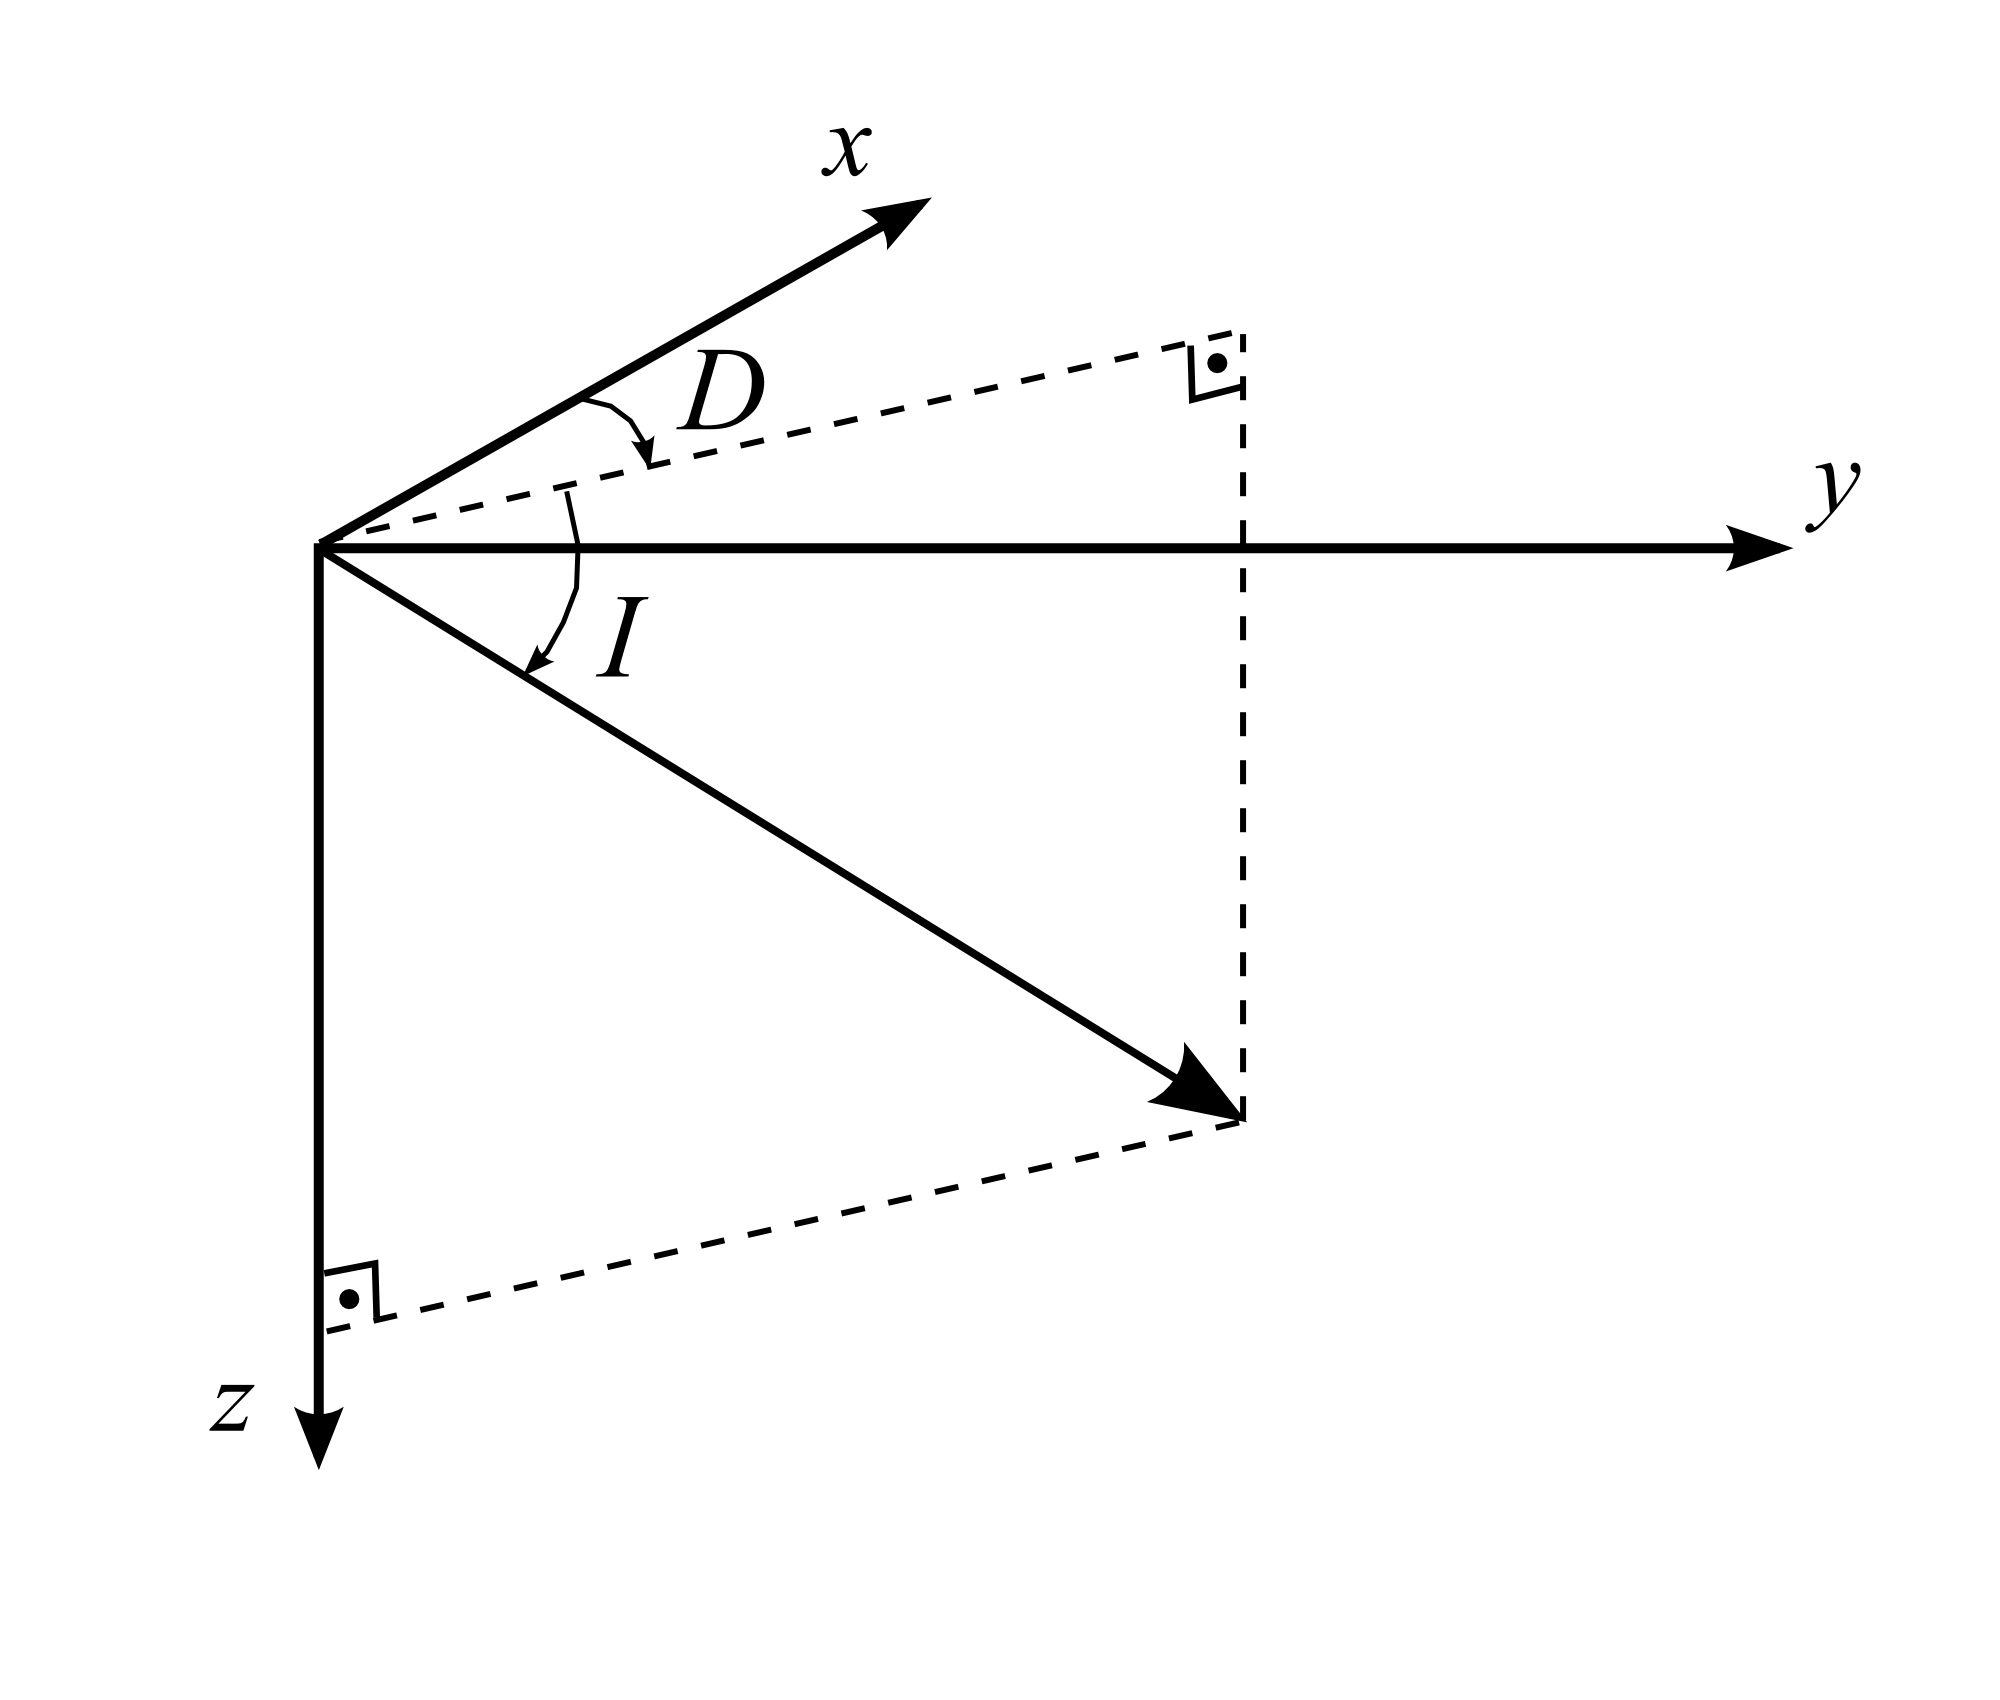
\includegraphics[scale=1]{Figs/Fig3.png}
    \caption{Representação esquemática de um vetor com declinação $D$ e inclinação $I$ referidas
        a um sistema de coordenadas Cartesianas com o eixo $x$ apontando para o norte geográfico,
        $y$ apontando para o leste e $z$ para baixo.}   
    \label{fig:fig3}
\end{figure}
%<== Figuras

A anomalia de campo total em uma determinada posição $(x_{i}, y_{i}, z_{i})$, $i = 1,...,N$,
da \'{a}rea de estudo é definida da seguinte forma:
\begin{equation}
\Delta T_{i} = \| \mathbf{F} + \mathbf{B}_{i} \| - \| \mathbf{F} \| \; ,
\label{eq:act-exata}
\end{equation}
em que $\mathbf{B}_{i}$ é a indução magn\'{e}tica produzida na posição $(x_{i}, y_{i}, z_{i})$
por corpos geol\'{o}gicos magnetizados em subsuperf\'{i}cie. Em geral, a seguinte relaç\~{a}o
\'{e} v\'{a}lida:
\begin{equation}
\| \mathbf{F} \| \gg \| \mathbf{B}_{i} \| \; , \; i = 1,...,N.
\label{eq:f-maior-maior-b}
\end{equation}
Esta relaç\~{a}o possibilita aproximar a anomalia de campo total $\Delta T_{i}$ 
(Eq. \ref{eq:act-exata}) por uma s\'{e}rie de Taylor, tal como será descrito a seguir.

\subsection{Anomalia de Campo Total aproximada}

Seja $f(\mathbf{p})$ uma funç\~{a}o escalar dada por:
\begin{equation}
\begin{split}
f(\mathbf{p}) & = \| \mathbf{p} \| \\
              & = \sqrt{\mathbf{p}^{\intercal} \mathbf{p}} \\
              & = p_{x}^{2} + p_{y}^{2} + p_{z}^{2} \; ,
\end{split}
\label{eq:funcao-norma-Euclidiana}
\end{equation}
em que $\mathbf{p}$ é um vetor dado por
\begin{equation}
\mathbf{p} = 
\left[
\begin{array}{c}
p_{x} \\
p_{y} \\
p_{z}
\end{array}
\right]_{3 \times 1} \; .
\label{eq:vetor-p}
\end{equation}
A funç\~{a}o $f(\mathbf{p})$ (Eq. \ref{eq:funcao-norma-Euclidiana}) representa a norma Euclidiana 
do vetor $\mathbf{p}$ (Eq. \ref{eq:vetor-p}), cujas componentes Cartesianas são $p_{x}$, 
$p_{y}$ e $p_{z}$. A funç\~{a}o pode ser expandida em torno de um ponto $\mathbf{p}_{0}$ 
por meio de uma s\'{e}rie de Taylor at\'{e} ordem 1 da seguinte forma:
\begin{equation}
f(\mathbf{p}_{0} + \Delta\mathbf{p}) \approx
f(\mathbf{p}_{0}) + 
\nabla f(\mathbf{p}_{0})^{\intercal} \Delta\mathbf{p} \; ,
\label{eq:funcao-f-Taylor}
\end{equation}
em que $\Delta\mathbf{p}$ é um vetor que representa uma pequena perturbaç\~{a}o
em torno de $\mathbf{p}_{0}$ $\--$ isto \'{e}, $\| \mathbf{p}_{0} \| \gg \| 
\Delta \mathbf{p} \|$ $\--$
e $\nabla f(\mathbf{p}_{0})$ \'{e} o vetor gradiente
de $f(\mathbf{p}_{0})$, que \'{e} definido como:
\begin{equation}
\nabla f(\mathbf{p}_{0}) =
\left[
\begin{array}{c}
\frac{\partial f(\mathbf{p}_{0})}{\partial p_{x}} \\
\frac{\partial f(\mathbf{p}_{0})}{\partial p_{y}} \\
\frac{\partial f(\mathbf{p}_{0})}{\partial p_{z}}
\end{array}
\right]_{3 \times 1} \; .
\label{eq:gradiente-f}
\end{equation}
Se derivarmos a Equaç\~{a}o \ref{eq:funcao-norma-Euclidiana} em relaç\~{a}o \`{a}s vari\'{a}veis
$p_{x}$, $p_{y}$ e $p_{z}$, podemos reescrever o vetor $\nabla f(\mathbf{p}_{0})$ da seguinte 
forma:
\begin{equation}
\begin{split}
\nabla f(\mathbf{p}_{0}) & = 
\dfrac{\mathbf{p}_{0}}{\sqrt{\mathbf{p}_{0}^{\intercal} \mathbf{p}_{0}}} \\
                         & = \hat{\mathbf{p}}_{0} \; ,
\end{split}
\label{eq:gradiente-f-2}
\end{equation}
sendo $\hat{\mathbf{p}}_{0}$ um vetor unit\'{a}rio com a mesma direç\~{a}o e sentido
do vetor $\mathbf{p}_{0}$. Substituindo esta express\~{a}o (Eq. \ref{eq:gradiente-f-2})
na Equaç\~{a}o \ref{eq:funcao-f-Taylor} temos que:
\begin{equation}
f(\mathbf{p}_{0} + \Delta\mathbf{p}) \approx
\| \mathbf{p}_{0} \| + 
\hat{\mathbf{p}}_{0}^{\intercal} \Delta\mathbf{p} \; .
\label{eq:funcao-f-Taylor-2}
\end{equation}
Utilizando esta aproximaç\~{a}o por s\'{e}rie de Taylor (Eq. \ref{eq:funcao-f-Taylor-2})
e considerando que a induç\~{a}o magn\'{e}tica $\mathbf{B}_{i}$, $i=1,...,N$ (Eq. 
\ref{eq:act-exata}) \'{e} uma pequena perturbaç\~{a} no campo geomagn\'{e}tico 
$\mathbf{F}$ (Eq. \ref{eq:campo-geomagnetico}), $\--$ ou seja, que a Equaç\~{a}o
\ref{eq:f-maior-maior-b} \'{e} v\'{a}lida $\--$ podemos aproximar a anomalia de campo
total $\Delta T_{i}$ (Eq. \ref{eq:act-exata}) pela seguinte express\~{a}o:
\begin{equation}
\begin{split}
\Delta T_{i}^{a} & = \| \mathbf{F}\| + \dfrac{\mathbf{F}^{\intercal}}
                     {\sqrt{\mathbf{F}^{\intercal} \mathbf{F}}} 
                     \mathbf{B}_{i} - \| \mathbf{F} \| \\
                 & = \hat{\mathbf{F}}^{\intercal} \mathbf{B}_{i} \; ,
\end{split}
\label{eq:act-aprox}
\end{equation}
em que $\hat{\mathbf{F}}$ é um vetor unit\'{a}rio com a mesma direç\~{a}o e sentido
do campo geomagn\'{e}tico $\mathbf{F}$ (Eq. \ref{eq:campo-geomagnetico}). Vale
ressaltar que esta aproximaç\~{a}o (Eq. \ref{eq:act-aprox}) da anomalia de campo 
total (Eq. \ref{eq:act-exata}) pressup\~{o}e a validade da relaç\~{a}o descrita pela
Equaç\~{a}o \ref{eq:f-maior-maior-b}. 

\begin{flushleft}
\dotfill
\end{flushleft}

\subsubsection{Exerc\'{i}cio}

Seja $\mathbf{B}$ um vetor $3 \times 1$ que representa a induç\~{a}o magn\'{e}tica produzida
por um corpo geol\'{o}gico em uma determinada posiç\~{a}o na superf\'{i}cie da Terra. Este
vetor pode ser escrito como:
\begin{equation}
\mathbf{B} = \| \mathbf{B} \| \, \hat{\mathbf{B}} \; ,
\label{eq:ex321-vetor-b}
\end{equation}
em que $\| \mathbf{B} \|$ \'{e} a intensidade de $\mathbf{B}$ e $\hat{\mathbf{B}}$ é um vetor unitário
dado por
\begin{equation}
\hat{\mathbf{B}} = \left[
\begin{array}{c}
cos(i) \, cos(d) \\
cos(i) \, sen(d) \\
sen(i)
\end{array}
\right] \; ,
\label{eq:ex321-versor-b}
\end{equation}
sendo $d$ e $i$ a declinação e a inclinação de $\mathbf{B}$, respectivamente, de 
acordo com a Figura \ref{fig:fig3}. Utilizando este vetor $\mathbf{B}$ (Eq. 
\ref{eq:ex321-vetor-b}) e um vetor $\mathbf{F}$ que descreva o campo geomagn\'{e}tico
\'{e} poss\'{i}vel calcular a anomalia de campo total $\Delta T$ (Eq. 
\ref{eq:act-exata}) e a anomalia de campo total aproximada $\Delta T^{a}$ (Eq. 
\ref{eq:act-aprox}). \'{E} de se esperar que, quanto maior a intensidade de $\mathbf{F}$,
menos deve ser a diferença entre  $\Delta T$ (Eq. \ref{eq:act-exata}) e $\Delta T^{a}$ 
(Eq. \ref{eq:act-aprox}). Sendo assim:

\begin{enumerate}

\item Defina valores para $\| \mathbf{B} \|$, $d$ e $i$ (Eqs. \ref{eq:ex321-vetor-b} 
      e \ref{eq:ex321-versor-b}) e calcule um vetor $\mathbf{B}$.

\item Defina valores para $D$ e $I$ (Eq. \ref{eq:versor-campo-geomagnetico}) e calcule
      um vetor unit\'{a}rio $\hat{\mathbf{F}}$.

\item Defina um conjunto de $N$ valores $F = \| \mathbf{F} \|$.
      Estes valores devem formar uma s\'{e}rie crescente, que começa com valores menores
      que $\| \mathbf{B} \|$ (definido no item 1) e terminam com valores muito maiores
      que $\| \mathbf{B} \|$ (definido no item 1).
      
\item Utilizando o vetor unit\'{a}rio $\hat{\mathbf{F}}$ definido no item 2 e cada um 
      dos $N$ valores $F$ definidos no item anterior, calcule um vetor $\mathbf{F}$.
      
\item Para cada um dos $N$ vetores $\mathbf{F}$ definidos no item anterior, calcule a
      anomalia de campo total $\Delta T$ (Eq. \ref{eq:act-exata}) e a anomalia de campo 
      total aproximada $\Delta T^{a}$ (Eq. \ref{eq:act-aprox}).
      
\item Faça um gr\'{a}fico da anomalia de campo total predita pelas Equaç\~{o}es \ref{eq:act-exata}
      e \ref{eq:act-aprox} em funç\~{a}o da razão $F/\| \mathbf{B} \|$.

\item A partir de qual valor $F/\| \mathbf{B} \|$ a diferença entre os valores preditos
      pelas Equaç\~{o}es \ref{eq:act-exata} e \ref{eq:act-aprox} é m\'{i}nima?

\end{enumerate}


\begin{flushleft}
\dotfill
\end{flushleft}

\bigskip
\bigskip

\end{document}
